%% -----------------------------------------------------------------
%% This file uses UTF-8 encoding
%%
%% For compilation use following command:
%% latexmk -pdf -pvc -bibtex --shell-escape thesis
%%
%% -----------------------------------------------------------------
%%                                     _     _      
%%      _ __  _ __ ___  __ _ _ __ ___ | |__ | | ___ 
%%     | '_ \| '__/ _ \/ _` | '_ ` _ \| '_ \| |/ _ \
%%     | |_) | | |  __/ (_| | | | | | | |_) | |  __/
%%     | .__/|_|  \___|\__,_|_| |_| |_|_.__/|_|\___|
%%     |_|                                          
%%
%% -----------------------------------------------------------------

\documentclass{kithesis}

% Additional packages
\usepackage[english,slovak]{babel}
\usepackage{blindtext}  % lorem ipsum
\usepackage{amssymb}
\usepackage{tikz}
\usepackage[cache=false]{minted}
\newenvironment{code}{\VerbatimEnvironment\begin{minted}{haskell}}{\end{minted}}

\newcommand*{\field}[1]{\mathbb{#1}}%
\usetikzlibrary{calc}
\usepackage{tkz-euclide}
\usetkzobj{all}
\usepackage{braket}

\usepackage{float}
% Variables
%\thesisspec{figures/thesisspec.png} 

\title{Measurement and interaction of quantum circutis}{Meranie a interakcia kvantových obvodov}

\author{Marián Sabat}
\supervisor{prof. Ing. Ján Kollár, CSc.} %veduci prace
%\consultant{Donald E. Knuth} %konzultant
\college{Techincal University of Kosice}{Technicka Univerzita v Kosiciach} %univerzita
\faculty{Faculty of Electrical Engineering and informatics}{Fakulta elektrotechniky a informatiky} %fakulta
\department{Department of Computers and Informatics}{Katedra počítačov a informatiky} %katedra
\departmentacr{DCI}{KPI} % skratka katedry
\thesis{Master thesis}{Diplomová práca} %typ prace
\submissiondate{1}{1}{2020}
\fieldofstudy{9.2.1 Informatika}
\studyprogramme{Informatika}
%\city{Košice} %mesto
\keywords{Quantum computers, measurement, Haskell, probability of quantum states}{Kvantové počítače, meranie, Haskell, pravdepodobnosť kvantových stavov}

\declaration{Vyhlasujem, že som záverečnú prácu vypracoval samostatne s 
použitím uvedenej odbornej literatúry.}

\abstract{
    % english 
	%\blindtext
The diploma thesis deals with the topic of measuring quantum circuits. 
This work explains the principle of measurement, which is used in the software 
solution. Also there is use of this program in several experiments that
 confirm its functionality. Chapter one describes the goal of this work in 
more detail. Mathematical theory necessary to understand the work is described 
in Chapter 2. The next two chapters build on this knowledge and describe the 
theory of quantum computers. Section The Probabilistic Analysis of quantum 
circuits points to problems that occur when trying to measure the states of 
quantum bits. Detaily processed experiments, in Chapter 6, show the 
functionality of the solution. Chapter 7 then
contains the design and implementation of a software solution for a 
probabilistic model
in Haskell. The Quantum Teleportation section lists more complex use
on a circuit with strongly entangled bits. In the end, all achievements are 
listed in results of this work.
}{
    % slovak 
	%\blindtext
Diplomová práca sa zaoberá témou merania kvantových obvodov. V práci je 
vysvetlený princíp merania, ktorý je využitý v programovom riešení. Ďalej sa
tento program využíta v niekoľkých experimentoch, ktoré potvrdzujú jeho
funkčnosť. Kapitola jeden detalnejšie popisuje cieľ tejto práce. Matematická
teória, nutná na pochopenie práce je rozpísaná v kapitole 2. Ďalšie dve
kapitoly nadvezujú na tieto poznatky a opisujú teóriu kvantových počítačov.
Časť Pravdepodobnostná analýza kvantových obvodov poukazuje na problémi, ktoré
nastávajú pri snahe merať stavy kvantových bitov. V kapitole 6 sú detailne 
spracované experimenty, ktoré zobrazujú funkčnosť riešenia. Kapitola 7 potom
obsahuje návrh a realizáciu programového riešenia pravdepodobnostného modelu
v jazyku Haskell. Časť Kvantová teleportácia uvádza zložitejšie využitie
na obvode so silno previazanými bitmi. V závere sú uvedené všetky dosiahnuté
výsledky tejto práce.
}

\acknowledgment{Na tomto mieste by som rád poďakoval svojmu vedúcemu práce za jeho čas, odborné vedenie počas riešenia mojej záverečnej práce a hlavne za jeho
železnú trpezlivosť.

Rovnako by som sa rád poďakoval svojim rodičom a priateľom za ich podporu a povzbudzovanie počas celého môjho štúdia.
    
%V neposlednom rade by som sa rád poďakoval pánom {\it Donaldovi E. Knuthovi} a {\it Leslie Lamportovi} za typografický systém \LaTeX, s ktorým som strávil množstvo nezabudnuteľných večerov.
}

\addbibresource{chapters/bibliography.bib}

% if you want to work only on selected chapters
%\includeonly{chapters/analyza} %,chapters/synteza}

% Load acronyms
\input{acronyms}

%% -----------------------------------------------------------------
%%          _                                       _   
%%       __| | ___   ___ _   _ _ __ ___   ___ _ __ | |_ 
%%      / _` |/ _ \ / __| | | | '_ ` _ \ / _ \ '_ \| __|
%%     | (_| | (_) | (__| |_| | | | | | |  __/ | | | |_ 
%%      \__,_|\___/ \___|\__,_|_| |_| |_|\___|_| |_|\__|
%%                                                      
%% -----------------------------------------------------------------

\begin{document}
%% Title page, abstract, declaration etc.:
\frontmatter{}

%% List of code listings, if you are using package minted
%\listoflistings

\pagenumbering{arabic}

%% Chapters
% !TEX root = ../thesis.tex

\chaptermark{Úvod}
\addcontentsline{toc}{chapter}{Úvod}

\chapter*{Úvod}

Často sa hovorí o konci platnosti Moorovho zákona. Je možné, že v blízkej
budúcnosti svet bude nútený zmentiť klasické počítače od základu. Jedným 
často spomínaným vývojovým schodom v tejto oblasti je kvantový počítač.
Pokusy využiť kvantovú fyziku v odbore počítačovej vedy možno nájsť už v
minulosti, no až v horizonte niekoľkých rokov nastal prelom a kvantové
počítače vznikajú po celom svete.

No napriek tomu stále chýba množstvo nástrojv, ktoré by sprístupnili vývoj
širšej verejnosti. Existujú voľne dostupné simulátory na generovanie kvantových
obvodov, ale od plne funkčných programov máme ešte ďaleko. Tento odbor je 
veľmi náročný a každý pokus zaberá množstvo času. 

Touto prácou sa pokúsime vylepšiť súčasnú situáciu. A to vytvorením nástroja,
ktorý by zlepšil porozumenie pri vykonávaní programov. I keď nepôjde o 
dokonale sofistikovaný simulátor kvantového počítača, napriek tomu porozumenie,
zrýchlenie a spríjemnenie vývoja programov pre tento druh počítačov môže 
priniesť nové pokroky v odvetví.

Bude v našom úmysle, čo najjednoduchšie vysvetliť princípy, ktoré sa skrývajú
za fungovaním kvantových počítačov. Naša práca ponúka teoretické minimum
nutné na porozumenie praktických experimentov a využíva ho pri priblížení
základných kvantových javoch, ako napríklad zvjazanie kvantových bitov, ktoré 
tvoria podstatu kvantových výpočtov ale aj pri zložitejších úkonoch ako 
kvantová teleportácia.


Čo je najdôležitejšie, pokúsime sa jasne a zrozumiteľne vysvetliť princíp
merania zmien stavov kvantových bitov. Poskytneme pohľad do matematického
aparátu, ktorý umožňuje simuláciu kvantových programov na klasických strojoch.
Priblížime vývoj pravdepodobnostného modelu vytvoreného vo funkcionálnom jazkyu
Haskell. A poskytneme komplexný návod na jeho použitie.

% !TEX root = ../thesis.tex

\chapter{Ciele prace (Formulacia ulohy)}

Prvou z častí, ktoré je nutné splniť je analýza princípov merania pri 
vykonávaní kvantových programov. Je nutné poskytnúť teoretické informácie
o spôsobe fungovania kvantových počítačov a vysvetliť matematické úkony,
doplnené o praktické príklady, nutné pri meraní zmeny stavov kvantových 
bitov.

Hlavným grom práce bude tvoriť návrh a implementácia zjednodušeného 
kvantového systému. Tento program bude schopný merať stav kvantového systému 
bez kolabovania bitov. Funkcionalita bude postavená na princípoch zýskaných
z analýzy.

Podstatnou funkcionalitou výsledného progamu bude grafické zobrazenie 
vypočítaných pravdepodobnosí stavov kvantových bitov a prehľad ako sa dané
bity menia počas behu programu.

%Text záverečnej práce musí obsahovať\/ kapitolu s~formuláciou úlohy resp. úloh riešených v~rámci záverečnej práce. V~tejto časti autor rozvedie spôsob, akým budú riešené úlohy a~tézy formulované v~zadaní práce. Taktiež uvedie prehľad podmienok riešenia.


% !TEX root = ../thesis.tex

\chapter{Matematicke zaklady kvantovych systemov}

\section{Matice}
\section{Komlexne cisla}
\section{Vektory}

% !TEX root = ../thesis.tex

\chapter{Teoreticke zaklady kvantovych systemov}

\section{Zakladne definicie}

\subsection{Hilbertov priestor ... atd}
\subsection{System s jednym kvantovym bitom}
\subsection{System s viacerymi kvantovymi bitmy}
\subsection{Princip merania}

% !TEX root = ../thesis.tex

\chapter{Kvantovy system}

\section{IBM QX}

\subsection{Stavy a ich zapis}
\subsection{Operacie kvantovych hradiel}

% !TEX root = ../thesis.tex

\chapter{Pravdepodobnostná analýza kvantových obvodov}
\label{pravAnalL}

V predošlých kapitolách bola vysvetlená problematika kvantových obvodov.
Našou úlohou je merať stavy kvantových bitov v rôznych časových okamihoch.
Je možné zostrojiť nekonečné množstvo rôznych kvantových obvodov,
a preto v tejto kapitole priblížime spôsob tohto merania.
Vo všeobecnosti môžme rozdeliť kvantové obvody na dva druhy, v ktorých 
meranie má iný charakter. Sú to obvody s nepreviazanými bitmi a obvody s 
previazanými kvantovými bitmi.

\section{Analýza nepreviazaných stavov}

\begin{figure} 
	\centering 
	\includegraphics[width=.4\textwidth]{figures/simpleCircuit2.png} 
	\caption{Jednotduchý kvantový obvod (namodelovaný v IBM Quantum Experience)}
    \label{obvod}
\end{figure}

Na obrázku \ref{obvod} je vygenerovaný jednoduchý kvantový obvod pomocou
nástroja IBM Quantum Experience. Označili sme dva časové úseky 
\(t_1\) a \(t_2\). V tomto obvode sú dva kvantové bity, ktoré prechádzajú 
hradlom CNOT. Pre 
zachovanie notácie budeme ďalej označovať tieto bity ako 
\(\psi_0\) a \(\psi_1\). Z kvantového obvodu je zrejmé, že v čase \(t_1\) 
sú oba kvantové bity v stave
\(\ket{0}\), to ale nebudeme brať v úvahu. Zaujíma nás pravdepodobnosť 
namerania stavov \(\ket{00}, \ket{01}, \ket{10}\) a \(\ket{11}\).

Vieme, že platí \(\ket{\psi_0} = \binom{\alpha_0}{\beta_0}\) a  
\(\ket{\psi_1} = \binom{\alpha_1}{\beta_1}\), a teda pre celkový stav \(\psi\) 
platí 
\[
\ket{\psi} = \ket{\psi_0} \otimes \ket{\psi_1} = \binom{\alpha_0}{\beta_0}
\otimes \binom{\alpha_1}{\beta_1} = 
\begin{pmatrix}
    \alpha_0\alpha_1 \\
    \alpha_0\beta_1 \\
    \beta_0\alpha_1 \\
    \beta_0\beta_1
\end{pmatrix}
\]
Z toho vyplíva, že celkový stav \(\ket{\psi}\) v čase \(t_1\) nadobúda 
hodnoty
\begin{itemize}
    \item[] \(\ket{00}\) s pravdepodobnosťou \(\Vert \alpha_0\alpha_1 \Vert^2\)
    \item[] \(\ket{01}\) s pravdepodobnosťou \(\Vert \alpha_0\beta_1 \Vert^2\)
    \item[] \(\ket{10}\) s pravdepodobnosťou \(\Vert \beta_0\alpha_1 \Vert^2\)
    \item[] \(\ket{11}\) s pravdepodobnosťou \(\Vert \beta_0\beta_1 \Vert^2\)
\end{itemize}

Toto tvrdenie platí, pretože platí 
\(\ket{\psi_0} = \alpha_0\ket{0} + \beta_0\ket{1}\), čiže 
\(|\alpha_0|^2 + |\beta_0|^2 = 1\), z čoho vyplíva, že 
\begin{itemize}
    \item[] \(\ket{\psi_0}\) nadobúda hodontu 0 s 
pravdepodobnosťou \(|\alpha_0|^2\) a 
    \item[] \(\ket{\psi_0}\) nadobúda hodontu 1 s 
pravdepodobnosťou \(|\beta_0|^2\).
\end{itemize}
Obdobne to platí aj pre \(\ket{\psi_1}\). K rovnakému záveru sa dopracujeme
aj pomocou 
\[\ket{\psi} = \ket{\psi_0} \otimes \ket{\psi_1} = 
(\alpha_0\ket{0} + \beta_0\ket{1}) \otimes  (\alpha_1\ket{0} + \beta_1\ket{1}) =
\]
\[
\alpha_0\alpha_1 (\ket{0} \otimes \ket{0}) +  
\alpha_0\beta_1 (\ket{0} \otimes \ket{1}) + 
\beta_0\alpha_1 (\ket{1} \otimes \ket{0}) + 
\beta_0\beta_1 (\ket{1} \otimes \ket{1}) 
\]
, čo by sme mohli vyjadriť aj iným zápisom ako 
\(
\alpha_{00}\ket{00} + \alpha_{01}\ket{01} + 
\alpha_{10}\ket{10} + \alpha_{11}\ket{11}
\), pričom súčet noriem musí byť rovný 1.
\[
|\alpha_{00}|^2 + |\alpha_{01}|^2 + |\alpha_{10}|^2 + |\alpha_{11}|^2 = 1\]

\section{Analýza previazaných stavov}

Pri meraní stavov v čase \(t_2\), už nemožno dostať výsledný stav \(\psi\)
priamim využitím tenzorového súčinu. Pri prechode hradom CNOT môžu nastať
dve situácie:
\begin{enumerate}
    \item Kvantový bit \(\psi_0\), ktorý je kontrólnym bitom, je v stave 
\(\ket{1}\) a teda nastane preklopenie bitu \(\psi_1\), čo je cieľoým bitom,
pomocou hradla X,
    \item Kvantový bit \(\psi_0\) nie je v stave \(\ket{1}\) a teda bit 
\(\psi_1\) pokračuje bez zmeny.
\end{enumerate}

Z toho je jasné, že v kažom prípade sa stav \(\ket{\psi_0}\) nemení no
stav \(\ket{\psi_1}\) nadobúda hodnotu:
\begin{itemize}
    \item \(\ket{\psi_1}\) s pravdepodobnosťou \(|\alpha_0|^2\),
    \item \(X\ket{\psi_1}\) s pravdepodobnosťou \(|\beta_0|^2\).
\end{itemize}
Berme v úvahu to, že v príklade sme využili hradlo CNOT. Pri pohľade na 
viacbitový systém s využitím haradla CCNOT, kde máme viacero kontrólnych bitov,
zisťujeme, že odvodzovanie je netriviálne a tento problém je nutné riešiť
pomocou pravdepodobnostného rozhodovacieho stromu (o tom v ďalších kapitolách).

% !TEX root = ../thesis.tex

\chapter{Meranie kvantových obvodov}

Jediným spôsobom ako zistiť skutočný stav kvnatového obvodu je meraním.
Merať možno všetky bity súčasne ako aj jednotlivé kvantové bity samostatne.

\section{Princíp merania kvantových obvodov}

Kvantový bit môže existovať v nekonečnom množstve stavov. Meranie si môžme 
predstaviť ako prevod stavov kvantových bitov do stavu klasického digitálneho
systému \cite{Nie10}. Pre príklad môžeme reprezentovať kvantový stav 
\(\alpha\ket{0} + \beta\ket{1}\) pomocou nulového a excitovaného stavu atómu.
Skutočný kvantový počítač by tak mohol merať tieto stavy. Pri meraní by 
daný atóm skolaboval do jedného zo stavov \(\ket{0}\) alebo \(\ket{1}\).
Pre kolabovanie samozrejme rovnako platí to, že do jednotlivých stavov by
sa atóm dostal s pravdepodobnosťami \(|\alpha|^2\) respektíve \(|\beta|^2\).


Pri každom fyzikálnom meraní nastáva určitá nepresnosť merania. Takisto 
pri meraní môže dokonca nastať zničenie obvodu. To vyplíva z toho, že pri
skolabovanom kvantovom bite nastáva zmena fizykálnych vlastností daného bitu. 

\section{Fiktívne meranie}

Našim cieľom je navrhnúť pravdepodobnostný model, ktorý by umožnil merať
stavy kvantových obvodov aj bez kolabovania jednotlivých kvantových bitov.

\subsection{Experiment 1}
Navrhnime kvantový obvod s dvoma bitmi. Označme ich \(\ket{\psi_0}\) a 
\(\ket{\psi_1}\). V prvom kroku aplikujeme Hadamardovo hrado na bit 
\(\ket{\psi_0}\). Nasledovať budú dve \(CNOT\) hradlá, s opačnými kontrólnymi 
a cieľovými bitmi. V IBM QX je tento obvod reprezenovaný ako 
\begin{code}
qreg q[2];
creg c[2];

h q[0];
cx q[0],q[1];
cx q[1],q[0];
\end{code}
Jeho grafické zobrazenie je na obrázku \ref{expr1_circuit}, aj s označenými
časovými úsekmi, v ktorých bude meraný stav systému. 

\begin{figure} 
	\centering 
	\includegraphics[width=.6\textwidth]{figures/expr1_circuit.png} 
	\caption{Obvod experimentu 1 s označenými časovými úsekmi meraní.}
    \label{expr1_circuit}
\end{figure}

\subsection*{Teoretická analýza}
Kvantové bity \(\ket{\psi_0}\) a \(\ket{\psi_2}\) sú definované ako 
\[\ket{\psi_0} = \alpha_0\ket{0} + \beta_0\ket{1}\]
\[\ket{\psi_1} = \alpha_1\ket{0} + \beta_1\ket{1}\]
, a teda je zrejmé, že v čase \(t_1\) pre celkový stav \(\ket{\psi}\) platí 
\[\ket{\psi} = \ket{\psi_0} \otimes \ket{\psi_1} = \alpha_0\alpha_1\ket{00} + \alpha_0\beta_1\ket{01} + \beta_0\alpha_1\ket{10} + \beta_0\beta_1\ket{11}\]

Z čoho jasne vyplíva, že systém nadobudne stav
    \begin{itemize}
        \item[] \(\ket{00}\) s pravdepodobnosťou \(|\alpha_0\alpha_1 |^2\)
        \item[] \(\ket{01}\) s pravdepodobnosťou \(| \alpha_0\beta_1 |^2\)
        \item[] \(\ket{10}\) s pravdepodobnosťou \(| \beta_0\alpha_1 |^2\)
        \item[] \(\ket{11}\) s pravdepodobnosťou \(| \beta_0\beta_1 |^2\) 
    \end{itemize}

Po prechode Hadamardovim hradlom, v čase \(t_2\) kvantové bity zmenia svoj stav
 na
\[\ket{\psi_0} = \frac{\alpha_0 + \beta_0}{\sqrt{2}}\ket{0} + \frac{\alpha_0 - \beta_0}{\sqrt{2}}\ket{1}\]
\[\ket{\psi_1} = \alpha_1\ket{0} + \beta_1\ket{1}\]

, a teda pre celkový stav \(\ket{\psi}\) bude platiť
\[\ket{\psi} = \frac{\alpha_0 + \beta_0}{\sqrt{2}}\alpha_1\ket{00} + \frac{\alpha_0 + \beta_0}{\sqrt{2}}\beta_1\ket{01} + \frac{\alpha_0 - \beta_0}{\sqrt{2}}\alpha_1\ket{10} + \frac{\alpha_0 - \beta_0}{\sqrt{2}}\beta_1\ket{11}\]

Kvantoý systém kolabuje v čase \(t_2\) do stavu
    \begin{itemize}
        \item[] \(\ket{00}\) s pravdepodobnosťou \(|\frac{\alpha_0 + \beta_0}{\sqrt{2}}\alpha_1|^2\)
        \item[] \(\ket{01}\) s pravdepodobnosťou \(|\frac{\alpha_0 + \beta_0}{\sqrt{2}}\beta_1|^2\)
        \item[] \(\ket{10}\) s pravdepodobnosťou \(|\frac{\alpha_0 - \beta_0}{\sqrt{2}}\alpha_1|^2\)
        \item[] \(\ket{11}\) s pravdepodobnosťou \(|\frac{\alpha_0 - \beta_0}{\sqrt{2}}\beta_1|^2\) 
    \end{itemize}

Zmena nastáva v čase \(t_3\), po prechode \(CNOT\) hradlom. Bit \(\ket{\psi_1}\)
bude preklopený len v prípade, že \(\ket{\psi_0}\) kolabuje do stavu 
\(\ket{1}\). A teda nastávajú dve možnosti. S pravdepodobnosťou 
\(|\frac{\alpha_0 + \beta_0}{\sqrt{2}}|^2\), ktorú označíme ako \(P^{t3}_1\) sa 
stavy kvantových bitov nezmenia
\[\ket{\psi_0} = \frac{\alpha_0 + \beta_0}{\sqrt{2}}\ket{0} + \frac{\alpha_0 - \beta_0}{\sqrt{2}}\ket{1}\]
\[\ket{\psi_1} = \alpha_1\ket{0} + \beta_1\ket{1}\]

Naopak, bit \(\ket{\psi_0}\) kolabuje do stavu \(\ket{1}\) s pravdepodobnosťou
\(|\frac{\alpha_0 - \beta_0}{\sqrt{2}}|^2\) (označme \(P^{t3}_{2}\)), a teda 
v tomto prípade nastáva zmena v kvantovom bite \(\ket{\psi_1}\)
\[\ket{\psi_1} = \beta_1\ket{0} + \alpha_1\ket{1}\]

Platí, že systém v čase \(t_3\) môže kolabovať do stavu
    \begin{itemize}
        \item[] \(\ket{00}\) s pravdepodobnosťou \((|\frac{\alpha_0 + \beta_0}{\sqrt{2}}\alpha_1|^2 \times P^{t3}_1) + (|\frac{\alpha_0 + \beta_0}{\sqrt{2}}\beta_1|^2 \times P^{t3}_{2})\)
        \item[] \(\ket{01}\) s pravdepodobnosťou \((|\frac{\alpha_0 + \beta_0}{\sqrt{2}}\beta_1|^2 \times P^{t3}_1 ) +(|\frac{\alpha_0 + \beta_0}{\sqrt{2}}\alpha_1|^2 \times P^{t3}_2)\)
        \item[] \(\ket{10}\) s pravdepodobnosťou \((|\frac{\alpha_0 - \beta_0}{\sqrt{2}}\alpha_1|^2 \times P^{t3}_1) +  (|\frac{\alpha_0 - \beta_0}{\sqrt{2}}\beta_1|^2 \times P^{t3}_2)\)
        \item[] \(\ket{11}\) s pravdepodobnosťou \((|\frac{\alpha_0 - \beta_0}{\sqrt{2}}\beta_1|^2 \times P^{t3}_1) +(|\frac{\alpha_0 - \beta_0}{\sqrt{2}}\alpha_1|^2 \times P^{t3}_2)\) 
    \end{itemize}


Poslendé meranie v tomto experimente je označené ako \(t_4\). Opäť nástáva
aktivácia \(CNOT\) hradla a teda podmienená zmena stavov kvantových bitov.
V každom prípade bit \(\ket{\psi_1}\) ostane nezmenený. No už teraz vychádzame 
z dvoch možností. Teda môžu nastať celkovo štyri pípady. V tabuľke 
\ref{expr1_t4_states} sú všetky možné zmeny stavov \(\ket{\psi_0}\) a
\(\ket{\psi_1}\).

\begin{table}
\centering
\begin{tabular}{|l|c|}
\hline
\textbf{Pravdepodobnosť} & \textbf{Stavy \(\ket{\psi_0}\) a \(\ket{\psi_1}\)} \\
\hline
\(P^{t4}_1 = |\frac{\alpha_0 + \beta_0}{\sqrt{2}}\alpha_1|^2\) & 
\(\ket{\psi_0} = \frac{\alpha_0 + \beta_0}{\sqrt{2}}\ket{0} + \frac{\alpha_0 - \beta_0}{\sqrt{2}}\ket{1}\) \\
& \(\ket{\psi_1} = \alpha_1\ket{0} + \beta_1\ket{1}\) \\
\hline

\(P^{t4}_2 = |\frac{\alpha_0 + \beta_0}{\sqrt{2}}\beta_1|^2\) & 
\(\ket{\psi_0} = \frac{\alpha_0 - \beta_0}{\sqrt{2}}\ket{0} + \frac{\alpha_0 + \beta_0}{\sqrt{2}}\ket{1}\) \\
& \(\ket{\psi_1} = \alpha_1\ket{0} + \beta_1\ket{1}\) \\
\hline

\(P^{t4}_3 = |\frac{\alpha_0 - \beta_0}{\sqrt{2}}\beta_1|^2\) & 
\(\ket{\psi_0} = \frac{\alpha_0 + \beta_0}{\sqrt{2}}\ket{0} + \frac{\alpha_0 - \beta_0}{\sqrt{2}}\ket{1}\) \\
& \(\ket{\psi_1} = \beta_1\ket{0} + \alpha_1\ket{1}\) \\
\hline

\(P^{t4}_4 = |\frac{\alpha_0 - \beta_0}{\sqrt{2}}\alpha_1|^2\) & 
\(\ket{\psi_0} = \frac{\alpha_0 - \beta_0}{\sqrt{2}}\ket{0} + \frac{\alpha_0 + \beta_0}{\sqrt{2}}\ket{1}\) \\
& \(\ket{\psi_1} = \beta_1\ket{0} + \alpha_1\ket{1}\) \\
\hline

\end{tabular}

\caption{\label{expr1_t4_states} Tabuľka stavov kvantových bitov a pravedpodobností
nastatia týchto stavov v čase \(t_4\) experimentu 1.}
\end{table}

Čiže celkový stav \(\ket{\psi}\) nadobudne stav
    \begin{itemize}
        \item[] \(\ket{00}\) s pravdepodobnosťou \\
\((|\frac{\alpha_0 + \beta_0}{\sqrt{2}}\alpha_1|^2 \times P^{t4}_1) + (|\frac{\alpha_0 - \beta_0}{\sqrt{2}}\alpha_1|^2 \times P^{t4}_2) + (|\frac{\alpha_0 + \beta_0}{\sqrt{2}}\beta_1|^2 \times P^{t4}_3) + (|\frac{\alpha_0 - \beta_0}{\sqrt{2}}\beta_1|^2 \times P^{t4}_4)\)

        \item[] \(\ket{01}\) s pravdepodobnosťou \\
 \((|\frac{\alpha_0 + \beta_0}{\sqrt{2}}\beta_1|^2 \times P^{t4}_1) + (|\frac{\alpha_0 - \beta_0}{\sqrt{2}}\beta_1|^2 \times P^{t4}_2) + (|\frac{\alpha_0 + \beta_0}{\sqrt{2}}\alpha_1|^2 \times P^{t4}_3) + (|\frac{\alpha_0 - \beta_0}{\sqrt{2}}\alpha_1|^2 \times P^{t4}_4)\)

        \item[] \(\ket{10}\) s pravdepodobnosťou \\ 
\((|\frac{\alpha_0 - \beta_0}{\sqrt{2}}\alpha_1|^2 \times P^{t4}_1) + (|\frac{\alpha_0 + \beta_0}{\sqrt{2}}\alpha_1|^2 \times P^{t4}_2) + (|\frac{\alpha_0 - \beta_0}{\sqrt{2}}\beta_1|^2 \times P^{t4}_3) + (|\frac{\alpha_0 + \beta_0}{\sqrt{2}}\beta_1|^2 \times P^{t4}_4)\)

        \item[] \(\ket{11}\) s pravdepodobnosťou \\
\((|\frac{\alpha_0 - \beta_0}{\sqrt{2}}\beta_1|^2 \times P^{t4}_1) + (|\frac{\alpha_0 + \beta_0}{\sqrt{2}}\beta_1|^2 \times P^{t4}_2) + (|\frac{\alpha_0 - \beta_0}{\sqrt{2}}\alpha_1|^2 \times P^{t4}_3) + (|\frac{\alpha_0 + \beta_0}{\sqrt{2}}\alpha_1|^2 \times P^{t4}_4)\)
    \end{itemize}

\subsection*{Výpočet pravdepodobností pomocou pravdepodobnostného modelu}
Pre použitie pravdepodobnostného modelu je nutné definovať obvod v jazyku 
Haskell. Vyjadrime jednotlivé hradlá a rozdeľme ich po vertikálnych leveloch.
\begin{code}
let l1 = Level [E, E] True
    l2 = Level [H, E] True
    l3 = Level [Cc, Ct] True
    l4 = Level [Ct, Cc] True
\end{code}
Pre meranie aj v čase \(t_1\), čiže ešte pred aktiváciou akéhokoľvek hradla,  
sme vložili jeden prázdny level navyše. Uložme tento obvod do spoločného listu
a definujme aj stromové štruktúry pre stavy a výsledky.
\begin{code}
c = [l1, l2, l3, l4]
st = StateTree 1 [q0, q0] []
rt = RT st []
\end{code}

Teraz už len spustime pravdepodobnostný model a uložme výsledky.
\begin{code}
let resultRT = processCircuit c rt
\end{code}

\begin{table}
\centering
\begin{tabular}{|c|}
\hline
1.0 \\ 
00 \\ 
\hline
\end{tabular}

\begin{tabular}{|c|c|}
\hline
0.5000000000000001 & 0.4999999999999999 \\ 
00 & 10 \\ 
\hline
\end{tabular}

\begin{tabular}{|c|c|c|c|}
\hline
0.25 & 0.2499999999999999 & 0.2500000000000001 & 0.25 \\ 
01 & 11 & 00 & 10 \\ 
\hline
\end{tabular}

\begin{tabular}{|c|c|c|c|c|c|}
\hline
0.25 & 0.2499999999999999 & 0.0 & 0.0 & 0.2500000000000001 & 0.25 \\ 
01 & 11 & 01 & 11 & 00 & 10 \\ 
\hline
\end{tabular}
\caption{\label{expr1_vystup} Výstup pravdepodobnostného modelu pre experiment 1
. Ohraničené riadky vymedzujú výsledky v jednotlivých časoch merania. Každá
bunka obsahuje pravdepodobnosť dosiahnutia stavu a daný stav systému.}
\end{table}

Pre vstupy kde na začiatku obvodu je \(\ket{\psi_0} = \ket{0}\) a zároveň
\(\ket{\psi_1} = \ket{0}\) nám model vypočítal výsledky, ktoré sú zaznamenané
v tabuľke \ref{expr1_vystup}. Každý ohraničený riadok predstavuje časový úsek.
Každá bunka potom obsahuje možný stav systému v daný časový úsek, kde horné
číslo je pravdepodobnosť dosiahnutia tohto stavu v rozmedzí \(0\) až \(1\) a 
spodná hodnota určuje daný stav v tvare \(\psi_0\psi_1\).

\begin{figure} 
	\centering 
	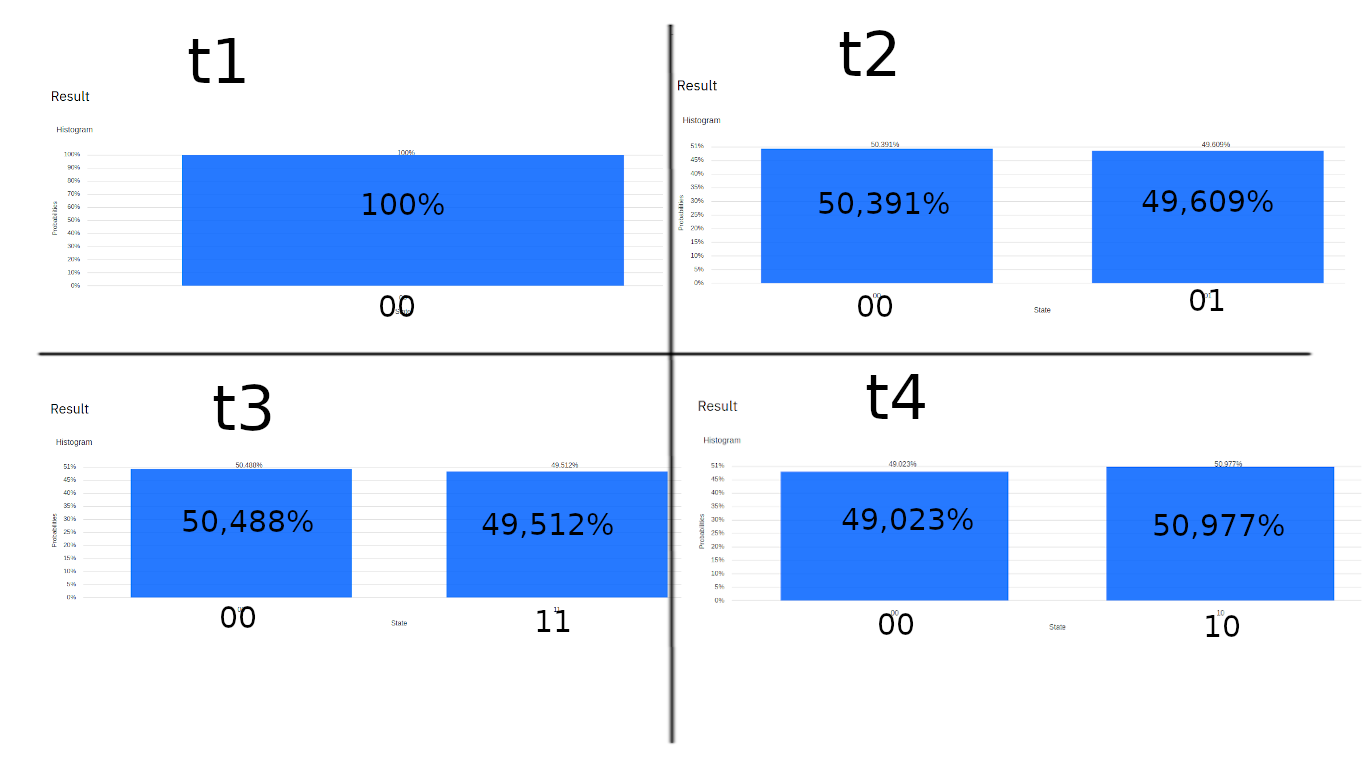
\includegraphics[width=.8\textwidth]{figures/expr1_qx_results.png} 
	\caption{Výsledky experimentu 1 z Quantum Experience so zvýraznenými 
údajmi.}

    \label{expr1_qx_results}
\end{figure}

Porovnajme naše výsledky so symulátorom IBM Quantum Experience. V IBM QX
bolo nutné vykonať štyri experimenty s rôznim časom merania, nakoľko tento
symulátor nepodporuje fiktívne meranie. Dosiahnuté výsledky sú na obrázku
\ref{expr1_qx_results}. Pripomeňme, že notácia dosiahnutých stavov v IBM QX
je \(\psi_1\psi_0\), teda v opačnom poradí ako zápis v našej tabuľke. V 
prvích dvoch merania sú výsledky totožné. Rozdiel nastáva pri prechode hradlom
\(CNOT\). Pravdepodobnostný model, ktorý využívame, funguje na istom 
matematickom aparáte. IBM QX je ale symulátor kantového počítača a teda môže 
brať do úvahy iné fyzikálne vlastnosti kvatových bitov, ktoré môžu vysvetľovať
rozdiel v našich výsledkoch.

\subsection{Experiment 2}
\subsection{Experiment 3}

% !TEX root = ../thesis.tex

\chapter{Pravdepodobnostný model kvantového výpočtu - návrh a realizácia}

Cieľom je vytvoriť v jazyku Haskell model, ktorý by dokázal merať stavy
kvantových bitov aj bez ich kolabovania. Na rozdiel od IBM Quantum
Experience tento model môže realizovať unitárne operácie aj paralelne.

\begin{figure}
	\centering 
	\includegraphics[width=.2\textwidth]{figures/navrh.png} 
	\caption{Konceptuálny návrh programu}
    \label{navrh}
\end{figure}


Pri pohľade na jednoduchý konceptuálny model (obrázok \ref{navrh}) je zrejmé,
čo chceme dosiahnuť. Na vstupe je očakávaný kvantový obvod. Samotný program
prebehne týmto obvodom ako interpreter a zároveň pomerá stavy na daných
miestach v obvode. Nakoniec vypíše výstup v zrozumiteľnej podobe.

\section{Definícia vstupu}

Celý kvantový obvod je možné rozdeliť do vertikálnych blokov alebo levelov.
Každý level obsahuje hradlá, ktorých počet je maximálne rovný počtu 
kvantových bitov, s~ktorými daný obvod pracuje. Ak v danom levely nechceme
aplikovať žiadnu operáciu nad bitom, môžme definovať prázdny element.
V obvode bude možné vyžiť osem základných hradiel, ktoré boli definované
v časti \ref{op_kvan_hradiel} Operácie kvantových hradiel, a hradlo 
C\textsuperscript{n}NOT.

\begin{code}
data Element = X
    | Y
    | Z
    | H
    | S
    | Sd
    | T
    | Td
    | Ct
    | Cc
    | E
\end{code}

Kvantový obvod môžeme definovať ako list levelov, pričom level je dátová
štruktúra, ktorá obsahuje list hradiel. Okrem hradiel každý level bude
obsahovať prepínač, ktorý signalizuje či má nastať fiktívne meranie po 
aktivácií hradiel v leveli.

\begin{code}
type LevelGates = [Element]
data Level = Level LevelGates Bool
\end{code}

\section{Pravdepodobnostný model}

\begin{figure}
	\centering 
	\includegraphics[width=.4\textwidth]{figures/circuit3.png} 
	\caption{Kvantový obvod s previazanými kvantovými bitmi.}
    \label{obvod}
\end{figure}

Pravdepodobnostný model možno vo funkčnosti prirovnať k interpreteru
kvantového obvodu. Tak ako bolo spomenuté v Pravdepodobnostnej analýze 
(kapitola \ref{pravAnalL}) je nutné brať v úvahu previazané a nepreviazané
kvantové bity. Previazanie je možné dosiahnuť hradlom CNOT (respektíve
C\textsuperscript{n}NOT). Našim cieľom nie je vytvoriť dokonalý interpreter,
z tohto dôvodu budeme využívať zjednodušené verzie týchto hradiel, čo znamená,
že ak kontrólne bity sú v stave \(\ket{1}\) tak cieľový kvantový bit bude 
preklopený hradom \(X\). V inom prípade nenastane zmena v stavoch.


Pravdepodobnostný model si uchováva stavy všetkých kvantových bitov a 
v~stromovej štruktúre. 
\begin{code}
type QBit = [[Complex Double]]
type States = [QBit]
type SubTrees = [StateTree]

data StateTree = StateTree Double States SubTrees
\end{code}

Pri prechode levelom si uloží nové stavy do listov
tohto stromu. Ak sa v leveli nachádzajú len obyčajné hradlá, vzniká len
jediný nový list. Rozdiel nastáva pri prechode hradlom CNOT. Je zrejmé, že 
toto hradlo musí rozvetvovať stromovú štruktúru na dva podstromy. Každý z 
podstromov je označený pravdepodobnosťou, s akou môže nastať daná zmena 
stavov. 

Pri meraní (fiktívnom meraní) sa spočítajú pravdepodobnosti všetkých listov
stromu a výsledky sa uložia do tabuľky. 
\begin{code}
data R = R Double [Int]
type T = [R]
type Ts = [T]
\end{code}
Dátová štruktúra R popisuje pravdepodobnosť dosiahnutia stavu, ktorý je 
reprezentovaný ako list celých čísel \(c_0c_1 \dots c_n\).
Pre lepšie pochopenie funkčnosti 
programu opíšeme príklad. Majme kvantový obvod, ktorý je definovaný na 
obrázku \ref{obvod}. Na vstupe máme dva kvantové bity v stavoch \(\ket{0}\).
Definujme všetky potrebné dátové štruktúry v jazyku Haskell. 

\begin{code}
l1 = Level [E, E] True
l2 = Level [H, E] True
l3 = Level [Cc, Ct] True
c = [l1, l2, l3]
st = StateTree 1 [q0, q0] []
rt = RT st []
\end{code}

Chceme merať v troch časových okamihoch, čo dosiahneme definovaním levelov
l1, l2 a l3. Každý level je označený na meranie pomocou True a využité hradlá
sú nasledovné:
\begin{itemize}
    \item E - prázdne
    \item H - Hadamardovo hradlo
    \item Cc - Kontrólny bit (angl. control bit) hradla CNOT
    \item Ct - Cieľový bit (angl. target bit) hradla CNOT
\end{itemize}

Pre ďalšie spracovanie spojíme levely  do jedného obvodu \(c\). Na ukladanie
stavov slúži stromová štruktúra StateTree. Jej definovaním hovoríme, že
počiatočné stavy sú q0, čo je označenie pre stav \(\ket{0}\). Pravdepodobnosť
dosiahnutia týchto stavov je 1 a zatiaľ neexistujú žiadne podstromy. Štruktúra
RT slúži na ukladanie výsledkov meraní. Spustením pravdepodobnostného modelu
dostaneme výslednú tabuľku typu RT.

\begin{code}
processRT = processCircuit c rt
\end{code}

Pričom štruktúra RT je definovaná ako
\begin{code}
data RT = RT StateTree Ts
\end{code}

\begin{figure}
	\centering 
	\includegraphics[width=.4\textwidth]{figures/ST.png} 
	\caption{Strom stavov (StateTree) po vykonaní kvantového obvodu,
kde hrany stromu sú označené pravdepodobnosťou dosiahnutia daného podstromu.}
    \label{stateTree}
\end{figure}

To ako sa menili stavy kvantových bitov môžeme vidieť na obrázku
\ref{stateTree}. Je zrejmé, že využitím operácie Hadarmardovho hradla nenastane
vetvenie stromu stavov. To isté ale už neplatí pre hradlo CNOT. Nakoľko stav
kontrólneho bitu \(\ket{+}\) má \(50\%\)-tnú šancu skolabovať do stavu 
\(\ket{0}\) ako aj do stavu \(\ket{1}\), tak je prirodzené, že strom stavov 
sa rozvetví a každý podstrom má pravdepodobnosť dosiahnutia približne \(0.5\).

Pri výpočte výsledkov je nutné započítať nie len pravdepodobnosti kolabovania
výsledných stavov ale aj pravdepodobnosti dosiahnutia podstromov, v ktorých 
sa dané stavy kvantových bitov nachádzajú. Meriame pravdepodobnosti kolabovania
bitov do stavov \(\ket{0}\) a \(\ket{1}\). Ide o dva stavy takže počet
kombinácií výsledkov je \(2^n\), kde \(n\) je počet kvantových bitov v obvode.
Teda pre dva bity možné kombinácie sú \(\ket{00}, \ket{01}, \ket{10}\) a
\(\ket{11}\). Vypočítajme výsledky pre level l3, čiže vychádzame z listov 
finálneho stromu stavov. Pre prvý list pravdepodobnosť dosiahnutia stavu:

\begin{itemize}
    \item \(\ket{00}\) je \(|\alpha_0\alpha_1|^2 = |\binom{1}{\sqrt{2}} \times
0|^2 = 0\)
    \item \(\ket{01}\) je \(|\alpha_0\beta_1|^2 = |\binom{1}{\sqrt{2}} \times
1|^2 = 0.5\)
    \item \(\ket{10}\) je \(|\beta_0\alpha_1|^2 = |\binom{1}{\sqrt{2}} \times
0|^2 = 0\)
    \item \(\ket{11}\) je \(|\beta_0\beta_0|^2 = |\binom{1}{\sqrt{2}} \times
1|^2 = 0.5\)
\end{itemize}

Pre druhý list obdobne platí to isté. Samozrejme, treba započítať aj
pravdepodobnosť vykonania podstromu. Preto všetky tieto pravdepodobnosti
kolabovania musíme vynásobiť príslušnými hodnotami. Teda dostávame výsledky:
\begin{itemize}
    \item \(\ket{00}\) dosiahneme s pravdepodobnosťou \(0.25\)
    \item \(\ket{01}\) dosiahneme s pravdepodobnosťou \(0.25\)
    \item \(\ket{10}\) dosiahneme s pravdepodobnosťou \(0.25\)
    \item \(\ket{11}\) dosiahneme s pravdepodobnosťou \(0.25\)
\end{itemize}

% !TEX root = ../thesis.tex

\chapter{Kvantová teleportácia}

Predstavme si situáciu, že chceme na diaľku komunikovať. Chceme poslať
informáciu o stave kvantového bitu. Zaznamenať komplexné číslo úplne presne 
na číslicovom počítači nejde, a teda nemožno poslať niekomu informáciu o 
presnom stave. Takisto platí, že kvantové bity je nemožné kopírovať či
klonovať. Spôsobom akým je možné riešiť tento problém je takzvaná kvantová
teleportácia.

Medzi účastníkov komunikácie sa rozdelí dvojica previazaných bitov. Ak tieto
kvantové bity nemeriame, zachovajú si svoj stav aj previazanie nehľadiac
na fyzickú vzdialenosť medzi nimi. Teda je možné komunikovať aj na diaľku.

Uveďme si všeobecne známy príklad na kvantovú teleportáciu. Povedzme, že 
Bob chce poslať kvantový bit Alici. Najprv je nutné aby obaja vlastnili
pár previazaných kvantových bitov. Ak teraz chce Bob poslať bit Alici, jediné
čo musí spraviť je aplikovať CNOT hradlo na svoj previazaný bit, ktorý bude 
kontrolovaný kvantovým bitom, ktorý chce odoslať. Potom aplikuje Hadamardovo
hradlo na odosielaný bit a pomeria obe bity. Alici odošle informáciu o
stavoch, ktoré kolabovaním dostal. Alica z tejto informácie vie, ako má použiť
hradlá X a Z, tak aby dosiahla rovnaký stav bitu, ktorý povodne vlastnil Bob.

Týmto spôsobom je možné informáciu poslať nakoľko sa jedná o celé čísla.
Takisto nie je porušená veta o kopírovaní ani klonovaní kvantových bitov, 
nakoľko Bob svoj bit stratil.

Ukážme si to na kvantovom obvode. Vytvoríme previazaný pár kvantových bitov
ako na obrázku \ref{tel_c1}. Povedzme, že bit \(q_1\) patrí Bobovi a \(q_2\)
je Alicin.

\begin{figure}[H]
	\centering 
	\includegraphics[width=.5\textwidth]{figures/tel_c1.png} 
	\caption{Previazanie kvantových bitov na kvantovú teleportáciu.}
    \label{tel_c1}
\end{figure}

Ako bolo spomenuté, na to aby mohol Bob poslať bit \(q_0\), musí aplikovať
CNOT a následne Hadamardovo hradlo, tak ako na obrázku \ref{tel_c2}.

\begin{figure}[H]
	\centering 
	\includegraphics[width=.5\textwidth]{figures/tel_c2.png} 
	\caption{Obvod popisujúci kvantovú teleportáciu.}
    \label{tel_c2}
\end{figure}

Bob pomeria svoje bity a pošle tieto merania Alici. Alica na základe týchto
meraní vie, že ak
\begin{itemize}
    \item[] Bobov bit \(q_0\) nadobudne stav \(1\), aplikuj hradlo \(Z\) na 
            \(q_2\)
    \item[] Bobov bit \(q_1\) nadobudne stav \(1\), aplikuj hradlo \(X\) na 
            \(q_2\)
\end{itemize}

\subsection*{IBM Quantum Experience výsledky}
Dokončime obvod. Povedzme, že posielame stav \(\ket{1}\), preto pridáme 
hradlo \(X\) na začiatok obvodu a plikujeme na \(q_0\). Na koniec pridáme 
podmienené aplikácie hradiel \(Z\) a \(X\). IBM QX podporuje variantu hradla
\(CNOT\), kde namiesto preklopenia \(X\) aplikujeme \(Z\). Výsledný obvod aj
s meraniami je na obrázku \ref{tel_qx_results}.

\begin{figure}
	\centering 
	\includegraphics[width=.7\textwidth]{figures/tel_qx_results.png} 
	\caption{Výsledky príkladku kvanovej teleportácie.}
    \label{tel_qx_results}
\end{figure}

Podľa výslekov je jasné, že teleportácia bola úspešná. Najhlavnejší bit 
všetkých výsledkov je \(1\). To znamená, že Alicin kvantový bit vždy nadobudne
taký stav aký mal pôvodne Bob, čo bolo \(\ket{1}\).

\subsection*{Pravdepodobnostný model}
Definujeme kvantový obvod pre program v jazyku Haskell.

\begin{code}
let l1 = Level [E, H, E] True
    l2 = Level [E, Cc, Ct] True
    l3 = Level [Cc, Ct, E] True
    l4 = Level [H, E, E] True
    c = [l1, l2, l3, l4]
    st = StateTree 1 [q1, q0, q0] []
    rt = RT st []
\end{code}
   
Bit \(q_0\) nastavýme na stav \(\ket{1}\), ostatné na \(\ket{0}\). V našom
pravdepodobnostnom modeli nejestvuje možnosť podmienených aplikácií hradiel,
tak si budeme musieť vystačiť s neúplnou teleportáciou.

Fiktívne meranie je nastavené za každým levelom, výsledky meraní su v tabuľke
\ref{tel_results}.

\begin{table}
\centering

\begin{tabular}{|c|c|}
\hline
0.50 & 0.49 \\ 
100 & 110 \\ 
\hline
\end{tabular}

\begin{tabular}{|c|c|c|c|}
\hline
0.25 & 0.249 & 0.25 & 0.25 \\ 
101 & 111 & 100 & 110 \\ 
\hline
\end{tabular}

\begin{tabular}{|c|c|c|c|c|c|c|c|}
\hline
0.25 & 0.249 & 0.0 & 0.0 & 0.25 & 0.25 & 0.0 & 0.0 \\ 
101 & 111 & 101 & 111 & 100 & 110 & 100 & 110 \\ 
\hline
\end{tabular}

\begin{tabular}{|c|c|c|c|c|c|c|c|}
\hline
0.125 & 0.1249 & 0.1249 & 0.1249 & 0.125 & 0.125 & 0.125 & 0.1249 \\ 
001 & 011 & 101 & 111 & 000 & 010 & 100 & 110 \\ 
\hline
\end{tabular}

\caption{\label{tel_results} Výsledky merania experimentu kvantovej
teleportácie pomocou
pravdepodobnostného modelu. Ohraničené riadky vymedzujú výsledky v jednotlivých
 časoch merania. Každá bunka obsahuje pravdepodobnosť dosiahnutia stavu a 
daný stav systému.}
\end{table}

Opäť pripomeňme, že poradie bitov vo výsledkoch z pravdepodobnostného modelu
a výsledkoch IBM QX je opačné. Pozornému oku neunikne, že v niektorých 
prípadoch výsledky po použití hradiel \(X\) a \(Z\) nebudú dávať správny 
výsledok. Je nutné podotknúť, že pravdepodobnostný model nepracuje až tak 
na základe vstupných stavov kvantových bitov v obvode ako na základe
matematikého modelu pravdepodobností dosiahnutia stavov \(\ket{0}\) a 
\(\ket{1}\). Takisto je vydno, že niektoré možnosti sú nedosiahnuteľné.
Teda výsledky pravdepodobnostného modelu sú narozdiel od IBM QX odvodzované od
všeobecných stavov kvantových bitov \(\ket{\psi}\) a vstupné hodnoty stavov
týchto bitov sú použité len na upravednie pravdepodobností do finálnej podoby.

% !TEX root = ../thesis.tex

\chapter{Celkové vyhodnotenie}

V tejto práci sme uviedli spôsob vykonávania a merania kvantových obvodov.
Využitím vedomostí z matematiky a funkcionálneho programovania sme úspešne 
navrhli a implementovali model pre počítanie fiktívnych meraní kvantových
bitov v kvantových obvodoch.

I keď nie je možné porovnávať simulátor kvantového stroje IBM Quantum
Experience s pravdepodobnostným modelom je nutné vyzdvihnúť fakt, že k
výsledkom a teda k predstave ako prebieha kvantový program sa dostaneme 
oveľa rýchlejšie. Na obrázku \ref{expr_time} sú zobrazené výpisy o dokončení
meraní experimentu v IBM QX. Pri experimentoch, ktoré sme vykonávali sme 
robili štyri fiktívne merania. Pre zistenie výsledkov zo simulátora kvantového
stroja, bolo nutné vykonať jednotlivé merania osobitne a to zabralo relatívne
veľa času. Ako je vidno na obrázku (\ref{expr_time}), vykonanie štyroch 
takýchto meraní trvalo viac ako dve minúty. Kde náš pravdepodobnostný model
vďaka tomu, že nemusí robiť reálne meranie ale len to fiktívne, vracia 
výsledky okamžite. 

\begin{figure}
	\centering 
	\includegraphics[width=.8\textwidth]{figures/time_expr.png} 
	\caption{Časy dokončení meraní experimetov.}
    \label{expr_time}
\end{figure}


Samozrejme, že ak potrebujeme presné merania, je lepšie použiť kompletný
simulátor. No výhodou nášho riešenia je zobrazenie zmien stavov kvantových
bitov. IBM QX dokáže zobraziť len skolabované výsledky meraní, i keď veľmi
presne, no niekedy je vhodnejšie vedieť stav ešte pred kolabovaním. Náš 
pravdepodobnosný model generuje stromovú štruktúru, v ktorej si zaznamenáva
priebežné stavy kvantových bitov. Získané stromy z našich experimentov sme 
pridali do príloh tejto práce.

Funkčnosť modelu sme otestovali na troch experimetoch. V každom experimente 
sme odvodili vzorce pre výpočet pravdepodobností kolabovania do jednotlivých
stavov pre všetky definované časové okamihy. Uviedli sme výsledky, ktoré 
sú dosiahnuteľné pomocou kvantového stroja IBM Quantum Experience. Nakoniec 
sme pre každý experiment uskutočnili meranie pomocou nášho pravdepodobnostného
modelu.

V neposlednej rade sme preskúmali aj možnosť využitia tohto pravdepodobnostného
modelu aj pri zložitejšom príklade, v ktorom prebiehal kvantový jaz zvaný
kvantová teleportácia.


%\include{chapters/vyprac}
%% !TEX root = ../thesis.tex

\chapter{Bezpečnostná analýza}


Pre dosiahnutie robustného riešenia sme museli zvážiť bezpečnostnú stránku programu.
Z tohto dôvodu sme vykonali bezpečnostnú analýzu.
Na vykonanie analýzy sme namodelovali diagram hrozieb pomocou nástroja Microsoft Threat Modeling Tool.
Na obrázku \ref{bez_di} je tento diagram.
Pomocou tohto programu sme veľmi rýchlo odhalili bezpečnostné hrozby, ktoré by mohli ohroziť vykonávanie nášho programu a dáta používateľa.
Ďalej v tejto kapytole popisujeme výstup našej analýzy.

\section{Zhrnutie modelu hrozby}

\begin{figure}[!t] 
	\centering 
	\includegraphics[width=.8\textwidth]{figures/diagram.png} 
	\caption{Diagram modelu hrozieb}
    \label{bez_di}
\end{figure}

\begin{enumerate}

\item \textbf{Spoofing cieľového dátového úložiska Graf stavov kvantovych bitov} \\ 
\textbf{Stav:} migrácia implementovaná \\
\textbf{Priorita:} vysoká
\begin{itemize}

\item[] \textbf{Kategória:} \\
Spoofing je, keď proces alebo entita je niečo iné ako jej nárokovaná identita. Medzi príklady patrí nahradenie procesu, súboru, webovej stránky alebo sieťovej adresy.
\item[] \textbf{Opis:} \\
Graf stavov kvantovych bitov môže útočník spoofovať, a to môže viesť k tomu, že údaje sa zapíšu do cieľa útočníka namiesto grafov kvantovych bitov. Zvážte použitie štandardného autentifikačného mechanizmu na identifikáciu cieľového úložiska údajov.
\item[] \textbf{Odôvodnenie:} \\
Použitie hashov na autentifikáciu.
\end{itemize}

\item \textbf{Potenciálna nadmerná spotreba zdrojov pre Prekladac (do grafu) alebo Graf stavov kvantovych bitov} \\
\textbf{Stav:} Vyžaduje sa vyšetrovanie \\
\textbf{Priorita:} vysoká 

\begin{itemize}
\item[] \textbf{Kategória:} \\
Odopretie služby nastane, keď proces alebo dátové úložisko nie je schopné obsluhovať prichádzajúce žiadosti alebo vykonávať špecifikácie.
\item[] \textbf{Opis:}  \\
Vykonáva prekladac (do grafu) alebo graf stavov kvantovych bitov výslovné kroky na kontrolu spotreby zdrojov? Útoky na spotrebu zdrojov môžu byť ťažko zvládnuteľné a niekedy je rozumné nechať OS robiť svoju prácu. Dávajte pozor, aby vaše žiadosti o zdroje neboli zablokované a aby nevypršali časové limity.
\item[] \textbf{Odôvodnenie:} \\
<neposkytuje sa migrácia>
\end{itemize}

\item \textbf{Podvádzanie externého subjektu - ľudského používateľa} \\
\textbf{Stav:} migrácia implementovaná \\
\textbf{Priorita:} vysoká 

\begin{itemize}
\item[] \textbf{Kategória:} \\
Spoofing je, keď proces alebo entita je niečo iné ako jej nárokovaná identita. Medzi príklady patrí nahradenie procesu, súboru, webovej stránky alebo sieťovej adresy.
\item[] \textbf{Opis:} \\
Ľudský užívateľ môže byť spoofovaný útočníkom a to môže viesť k neoprávnenému prístupu k interpretátoru kvantoveho obvodu. Zvážte použitie štandardného autentifikačného mechanizmu na identifikáciu externej entity.
\item[] \textbf{Odôvodnenie:} \\
Použitie autentifikácie.
\end{itemize}

\item \textbf{Nadväznosť pomocou zosobnenia} \\
\textbf{Stav:} migrácia implementovaná \\
\textbf{Priorita:} vysoká

\begin{itemize}
\item[] \textbf{Kategória:} \\
Subjekt používateľa získava zvýšenú spôsobilosť alebo privilégium využitím chyby implementácie.
\item[] \textbf{Opis:} \\
Interpreter kvantoveho  obvodu môže byť schopný zosobniť kontext ľudského používateľa, aby získal ďalšie privilégiá.
\item[] \textbf{Odôvodnenie:} \\
ACL
\end{itemize}

\item \textbf{Spoofing procesu interpretera kvantoveho obvodu} \\
\textbf{Stav:} migrácia implementovaná \\
\textbf{Priorita:} vysoká

\begin{itemize}
\item[] \textbf{Kategória:} \\
Spoofing je, keď proces alebo entita je niečo iné ako jej nárokovaná identita. Medzi príklady patrí nahradenie procesu, súboru, webovej stránky alebo sieťovej adresy.
\item[] \textbf{Opis:} \\
Interpreter kvantoveho obvodu môže útočník spoofovať, čo môže viesť k poskytovaniu informácií ľudským používateľom. Zvážte použitie štandardného autentifikačného mechanizmu na identifikáciu cieľového procesu.
\item[] \textbf{Odôvodnenie:} \\
Použitie autentifikácie
\end{itemize}

\item \textbf{Potenciálne nedostatočné overenie vstupu pre Interpreter kvantoveho obvodu} \\
\textbf{Stav:} migrácia implementovaná \\
\textbf{Priorita:} vysoká

\begin{itemize}
\item[] \textbf{Kategória:} \\
Manipulácia je akt zmeny bitov. Manipulácia s procesom zahŕňa zmenu bitov v bežiacom procese. Podobne manipulácia s dátovým tokom zahŕňa zmenu bitov na drôte alebo medzi dvoma bežiacimi procesmi.
\item[] \textbf{Opis:} \\
Údajom, ktorý tečie cez Kvantovy obvod, môže útočník zmanipulovať. Môže to viesť k odmietnutiu služobného útoku na tlmočníka kvantového rozsahu alebo k zvýšeniu výsadného privilégia proti tlmočníkovi kvantového množstva alebo k sprístupneniu informácií interpretom kvantového množstva. Opomenutie overiť, či je vstup očakávaný, je hlavnou príčinou veľmi veľkého množstva problémov, ktoré možno zneužiť. Zvážte všetky cesty a spôsob spracovania údajov. Overte správnosť všetkých vstupov pomocou schváleného prístupu na overenie vstupu do zoznamu.
\item[] \textbf{Odôvodnenie:} \\
Validácia vstupu.
\end{itemize}

\item \textbf{Potenciálne odmietnutie údajov Interpretera kvantového obvodu} \\
\textbf{Stav:} migrácia implementovaná \\
\textbf{Priorita:} vysoká

\begin{itemize}
\item[] \textbf{Kategória:} \\
Hrozby odmietnutia zahŕňajú protivníka, ktorý popiera, že sa niečo stalo.
\item[] \textbf{Opis:} \\
Interpreter kvantoveho obvodu tvrdí, že nedostal údaje zo zdroja mimo hranice dôveryhodnosti. Zvážte použitie protokolovania alebo auditu na zaznamenanie zdroja, času a súhrnu prijatých údajov.
\item[] \textbf{Odôvodnenie:} \\
Audit vstupov.
\end{itemize}

\item \textbf{Sniffing toku údajov} \\
\textbf{Stav:} migrácia implementovaná \\
\textbf{Priorita:} vysoká

\begin{itemize}
\item[] \textbf{Kategória:} \\ 
Zverejňovanie informácií nastane, keď ich môže prečítať neoprávnená strana.
\item[] \textbf{Opis:} \\
Údaj, ktorý tečie cez Kvantovy obvod, môže útočník vyvolať. V závislosti od toho, aký typ údajov môže útočník prečítať, možno ho použiť na útok na iné časti systému alebo jednoducho na odhalenie informácií vedúcich k porušeniu súladu. Zvážte šifrovanie toku údajov.
\item[] \textbf{Odôvodnenie:} \\ 
Ručné zadávanie.
\end{itemize}

\item \textbf{Potenciálne zlyhanie procesu alebo zastavenie Interpretera kvantoveho obvodu} \\ 
\textbf{Stav:} migrácia implementovaná \\
\textbf{Priorita:} vysoká

\begin{itemize}
\item[] \textbf{Kategória:} \\
Odopretie služby nastane, keď proces alebo dátové úložisko nie je schopné obsluhovať prichádzajúce žiadosti alebo vykonávať špecifikácie.
\item[] \textbf{Opis:} \\ 
Tlmočník kvantoveho signálu havaruje, zastavuje, ukončuje alebo beží pomaly; vo všetkých prípadoch porušujúcich metriku dostupnosti.
\item[] \textbf{Odôvodnenie:} \\
Využívanie kvót na predchádzanie veľkým vstupom.
\end{itemize}

\item \textbf{Tok údajov Kvantový obvod je potenciálne prerušený} \\
\textbf{Stav:} migrácia implementovaná \\
\textbf{Priorita:} vysoká

\begin{itemize}
\item[] \textbf{Kategória:} \\
Odopretie služby nastane, keď proces alebo dátové úložisko nie je schopné obsluhovať prichádzajúce žiadosti alebo vykonávať špecifikácie.
\item[] \textbf{Opis:} \\
Externý agent preruší údaje tečúce cez hranice dôveryhodnosti v oboch smeroch.
\item[] \textbf{Odôvodnenie:} \\
Validácia používateľa
\end{itemize}

\item \textbf{Interpreter kvantoveho obvodu môže byť predmetom zvýšenia oprávnenia pomocou vzdialeného vykonávania kódu} \\
\textbf{Stav:} migrácia implementovaná \\
\textbf{Priorita:} vysoká

\begin{itemize}
\item[] \textbf{Kategória:} \\
Subjekt používateľa získava zvýšenú spôsobilosť alebo privilégium využitím chyby implementácie.
\item[] \textbf{Opis:} \\ 
Ľudský užívateľ môže byť schopný diaľkovo vykonať kód pre tlmočníka kvantoveho kontroly.
\item[] \textbf{Odôvodnenie:} \\ 
Validácia vstupu.
\end{itemize}

\item \textbf{Vyzdvihnutie zmenou realizačného toku v Interpretore kvantoveho obvodu}  \\
\textbf{Stav:} migrácia implementovaná \\
\textbf{Priorita:} vysoká

\begin{itemize}
\item[] \textbf{Kategória:}  \\
Subjekt používateľa získava zvýšenú spôsobilosť alebo privilégium využitím chyby implementácie.
\item[] \textbf{Opis:} \\ 
Útočník môže preniesť údaje do kvantového interpreta Interpreter, aby zmenil tok vykonávania programu v Interpretore kvantového obvodu podľa výberu útočníka.
\item[] \textbf{Odôvodnenie:} \\ 
Overenie vstupných údajov.
\end{itemize}

\item \textbf{Vyzdvihnutie pomocou zosobnenia} \\ 
\textbf{Stav:} migrácia implementovaná \\
\textbf{Priorita:} vysoká

\begin{itemize}
\item[] \textbf{Kategória:} \\
Subjekt používateľa získava zvýšenú spôsobilosť alebo privilégium využitím chyby implementácie.
\item[] \textbf{Opis:} \\
Prekladač (do grafu) môže byť schopný zosobniť kontext interpretátora kvantovehobvodu, aby získal ďalšie privilégium.
\item[] \textbf{Odôvodnenie:} \\
Nastavenie povolení pre Prekladač (do grafu).
\end{itemize}

\end{enumerate}

\section{Zhrnutie}

Pri analýze sme odhalili 13 hrozieb.
Z hoto sa nám úspešne podarilo vyriešiť 12.
Pomocou tejto metódy sa nám veľmi rýchlo podarilo nájsť a eliminovať bezpečnostné nedostatky nášho programu.


%% !TEX root = ../thesis.tex

\chapter{Celkové vyhodnotenie}

V tejto práci sme uviedli spôsob vykonávania a merania kvantových obvodov.
Využitím vedomostí z matematiky a funkcionálneho programovania sme úspešne 
navrhli a implementovali model pre počítanie fiktívnych meraní kvantových
bitov v kvantových obvodoch.

I keď nie je možné porovnávať simulátor kvantového stroje IBM Quantum
Experience s pravdepodobnostným modelom je nutné vyzdvihnúť fakt, že k
výsledkom a teda k predstave ako prebieha kvantový program sa dostaneme 
oveľa rýchlejšie. Na obrázku \ref{expr_time} sú zobrazené výpisy o dokončení
meraní experimentu v IBM QX. Pri experimentoch, ktoré sme vykonávali sme 
robili štyri fiktívne merania. Pre zistenie výsledkov zo simulátora kvantového
stroja, bolo nutné vykonať jednotlivé merania osobitne a to zabralo relatívne
veľa času. Ako je vidno na obrázku (\ref{expr_time}), vykonanie štyroch 
takýchto meraní trvalo viac ako dve minúty. Kde náš pravdepodobnostný model
vďaka tomu, že nemusí robiť reálne meranie ale len to fiktívne, vracia 
výsledky okamžite. 

\begin{figure}
	\centering 
	\includegraphics[width=.8\textwidth]{figures/time_expr.png} 
	\caption{Časy dokončení meraní experimetov.}
    \label{expr_time}
\end{figure}


Samozrejme, že ak potrebujeme presné merania, je lepšie použiť kompletný
simulátor. No výhodou nášho riešenia je zobrazenie zmien stavov kvantových
bitov. IBM QX dokáže zobraziť len skolabované výsledky meraní, i keď veľmi
presne, no niekedy je vhodnejšie vedieť stav ešte pred kolabovaním. Náš 
pravdepodobnosný model generuje stromovú štruktúru, v ktorej si zaznamenáva
priebežné stavy kvantových bitov. Získané stromy z našich experimentov sme 
pridali do príloh tejto práce.

Funkčnosť modelu sme otestovali na troch experimetoch. V každom experimente 
sme odvodili vzorce pre výpočet pravdepodobností kolabovania do jednotlivých
stavov pre všetky definované časové okamihy. Uviedli sme výsledky, ktoré 
sú dosiahnuteľné pomocou kvantového stroja IBM Quantum Experience. Nakoniec 
sme pre každý experiment uskutočnili meranie pomocou nášho pravdepodobnostného
modelu.

V neposlednej rade sme preskúmali aj možnosť využitia tohto pravdepodobnostného
modelu aj pri zložitejšom príklade, v ktorom prebiehal kvantový jaz zvaný
kvantová teleportácia.

% !TEX root = ../thesis.tex

\chapter{Záver}



% good linebraking of bibtex url
\setcounter{biburllcpenalty}{7000}
\setcounter{biburlucpenalty}{8000}

%% The bibliography
\phantomsection
\addcontentsline{toc}{chapter}{Literatúra}
\printbibliography[title={Literatúra}]

% List of acronyms
\printglossary[type=\acronymtype,title={\acrlistname}]

%% Appendix
% !TEX root = ../thesis.tex

\chapter*{Zoznam príloh}
\addcontentsline{toc}{chapter}{Zoznam príloh}

\begin{description}
    \item[Príloha A] Používateľská príručka
    \item[Príloha B] Systémová príručka
    \item[Príloha C] CD médium -- záverečná práca v~elektronickej podobe,
    
\end{description}

\appendix
\renewcommand\chaptername{Príloha}
% !TEX root = ../thesis.tex

\chapter{Používateľská príručka}

\section{Funkcia programu}

Program slúži na meranie kvantového obvodu. Do programu je nutné vložiť 
definíciu kvanotvého obvodu aj s označenými časmi merania. Program vygeneruje
latexové súbory pripravené na preklad pomocou laxeového prekladača. 
Vygenerované sú dva súbory
\begin{enumerate}
    \item Strom zmien stavov kvantových bitov (zn. 1),
    \item Tabuľka výsledkov fiktívnych meraní v daných časových úsekoch (zn. 2).
\end{enumerate}

\section{Systémové požiadavky}

Pre spustenie programu je nutné mať nainštalované: 
\begin{itemize}
    \item interpreter jazyka Haskell,
    \item latex.
\end{itemize}

\section{Inštalácia programu}

Samotný program nie je nutné nijako inštalovať. Programové skripty sú v 
adresáry program, pripravené na spustenie. Je ale nutné si pripraviť prostredie.
Pre inštaláciu jazyka Haskell postupujte podľa návodu na oficiálnej 
stránke \url{www.haskell.org}. Pre operačný systém linux použite svojho
správcu balíkov a nainštalujte haskell-platform. Príklad pre Ubuntu:

\begin{code}
sudo apt-get install haskell-platform
\end{code}

Na preklad výstupu do formátu .pdf je nutné použiť latex. Pre linux je
inštalácia jednoduchá, pomocou správcu balíkov nainštalujte texlive. Príklad
pre Ubuntu:

\begin{code}
sudo apt-get install texlive
\end{code}

Pre inštaláciu na Windows postupujte podľa pokynov na \url{http://www.tug.org/texlive/}. Alebo využite online nástroj Overleaf na \url{https://www.overleaf.com/}.

\section{Spustenie programu}

Pre definovanie kvantového obvodu je nutné upraviť súbor QWriter.hs. Vo 
funkcii main sú zakomentované štyry definície obvodov, ktoré boli použité 
v experimentoch diplomovej práce. Odkomentujte jeden alebo definujte nový
obvod rovnakým spôsobom. 

\begin{enumerate}
    \item Nadefinujte vertikálne levely (odporúčanie: pomenujte ich l1..ln),
    \item Uložte levely do listu ako premennú c,
    \item Definujte strom stavov ako premennú st
    \item Definujte tabuľku výsledkov ako rt.
\end{enumerate}

Definícia levelu obsahuje konštruktor Level, list hradiel v danom vertikálnom
levely (E - emplty, X, Y, Z, H, S, Sd, T, Td, Ct - cieľový bit CNOT hradla, 
Cc - kontrólny bit CNOT hradla) a indikátor, či má byť vykonané fiktívne
meranie \underline{za} daným levelom. Príklad:

\begin{code}
Level [E, H, X] True
\end{code}

Definícia stromu stavov obsahuje konštruktor StateTree, počiatočnú 
pravdepodobnosť (odporúčanie: nastaviť na 1), list počiatočných stavov
kvantových bitov (q1, q0, qP, qM, qR, qL alebo ľubovoľný stav definovaný
ako [[Complex Double]], príklad [[0.0 :+ 0.0],[1.0 :+ 0.0]]). 
Veľkosť tohto listu určuje počet kvantových bitov v obvode. Posledný prvok
definície stromu stavov je list podstromov (odporúčanie: nastaviť prázdny list).
Príklad:

\begin{code}
StateTree 1 [q0, q1] []
\end{code}

Definícia tabuľky výsledkov obsahuje konštruktor RT, strom stavov a list 
reprezentujúci samotnú tabuľku (odporúčanie: nastaviť prázdny list). Príklad:

\begin{code}
RT st []
\end{code}

% !TEX root = ../thesis.tex

\chapter{Systémová príručka}
%QCircuits.hs  
%QDefinitions.hs
%QEntanglement.hs  
%QMatrix.hs  
%QOperations.hs  
%QWriter.hs

Všetky potrebné skripty sa nachádzajú v adresáry program. Pri načítaní modulu
QWriter sa automaticky načítajú aj ostatné. 
\begin{itemize}
    \item QCircuits.hs - obsahuje pravdepodobnostý model a celú logiku merania,
    \item QDefinitions.hs - obsahuje definície základných kvantových stavov a
hradiel,
    \item QEntanglement.hs - obsahuje funkcie pre výpočet alfa a beta normy,
    \item QMatrix.hs - obsahuje oprerácie pre prácu s maticami,
    \item QOperations.hs - obsahuje definície operácií s kvanotvými bitmi
    \item QWriter.hs - obsahuje funkciu main a proces prekladu a zápisu do
latexu.
\end{itemize}

\section{Popis algoritmu pravdepodobnostného modelu}



% zivotopis autora
%\curriculumvitae\protect
%Táto časť\/ je nepovinná. Autor tu môže uviesť\/ svoje biografické
%údaje, údaje o~záujmoch, účasti na~projektoch, účasti na~súťažiach,
%získané ocenenia, zahraničné pobyty na~praxi, domácu prax, publikácie
%a~pod.

\end{document}
